\documentclass{minimal}

\usepackage{amsmath}
\usepackage{amssymb}
\usepackage{bm}
\usepackage{graphicx}

\DeclareMathOperator*{\argmax}{argmax}
\DeclareMathOperator*{\argmin}{argmin}

\begin{document}

\textbf{Linear classifiers}

Linear discriminant analysis (LDA)

Logistic regression

Support vector machine (SVM)

\medskip

\textbf{LDA}

Assume classes are multivariate Gaussian with common covariance matrix $\mathbf{\Sigma}$

It can be shown that under these assumptions the decision boundary between any
two classes is linear, i.e. a hyperplane in $\mathbb{R}$.

\smallskip

$w$ is a weight vector that defines a projection into a 1-dimensional subspace.
Then, in that sub-space, we set a threshold $t$ as the boundary between the two
classes. 

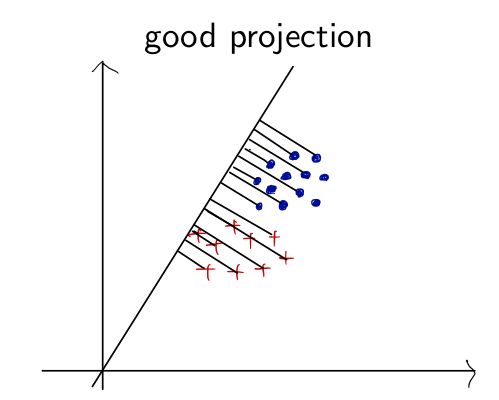
\includegraphics[scale=0.25]{lda}

Fisher's optimal projection: maximize between-class variance relative
to within-class variance. In other words: projected class centroids are far
apart, projected data are close to centroids.

$$
\hat{w} = \argmax_{w \in \mathbb{R}^d} \frac{w'\mathbf{B}w}{w'\mathbf{W}w}
$$

$$
\mathbf{B} = \sum_c (\bm{\mu}_c - \bar{\mathbf{x}}) (\bm{\mu}_c -
\bar{\mathbf{x}})'
$$
$$
\mathbf{W} = \sum_c \sum_{i \in c}(\mathbf{x}_i - \bm{\mu}_c) (\mathbf{x}_i -
\bm{\mu}_c)'
$$

\smallskip

Because $w$ is invariant to rescaling, we can choose $w$ such that
$w'\mathbf{W}w=1$, leading to:

$$
w^* = \argmax_w w'\mathbf{B}w 
$$
\begin{center}
s.t.
\end{center}
$$
w'\mathbf{W}w=1
$$

This is a generalized eigenvalue problem, with $w$ given by the largest
eigenvalue of $\mathbf{W}^{-1}\mathbf{B}$

\smallskip

If we assume Gaussian class densities and common covariance matrix
$\mathbf{\Sigma}$, then LDA is optimal (equivalent to Bayes).

\medskip

\textbf{Interlude: Lagrangian optimization}

Suppose that we have a standard optimization problem with $m$ inequality and/or
$p$ equality constraints:

\smallskip

Minimize $f_0(x)$

s.t. $f_i(x) \leq 0, \quad i=1...m$

$h_i(x)=0, \quad i = 1...p$

The Lagrangian is:
$$
L(x, \lambda, v) = f_0(x) + \sum_{i=1}^m \lambda_if_i(x) + \sum_{i=1}^p v_i
h_i(x)
$$

The dual function is the minimum value of the Lagrangian over $x$:
$$
g(\lambda, v) = \inf_x L(x, \lambda, v)
$$

This function is concave, even if the original problem is not convex. It also is
always less than or equal to the original objective function evaluated at its
optimal value. Putting these together, if we maximize $\lambda$ and $v$ in the dual, it is the same
as minimizing $x$ in the primal.

\medskip

\textbf{Logistic}

Same as usual. Estimate using MLE. Can add a regularizer. Often outperforms LDA
because it doesn't have squared error (bad). Example:

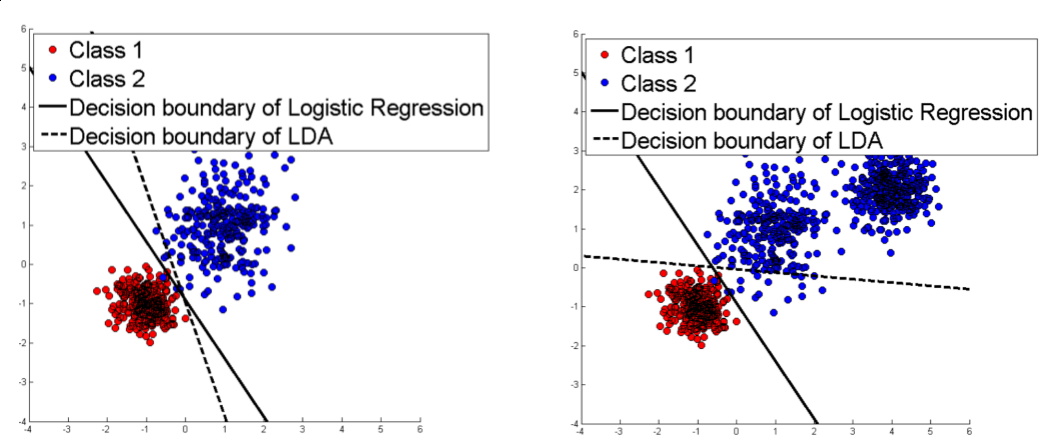
\includegraphics[scale=0.25]{log}

\medskip

\textbf{SVM}

Key advantages: no distribution assumptions and data compression (classification
only depends on a relatively small subset of overall data).

\smallskip

\textit{Hard margin}

Data must be linearly separable.

We want to construct a decision hyperplane $H_{w_0 + \langle w, x \rangle}$. 

Notation:
$w_0 + \langle w, x \rangle = \mathbf{w}^T\mathbf{X} + b = \sum w_ix_i + b$. For
example, fo line $3x+2$, $w=3$ and $w_0 = 2$.

We will require $w$ to be \textit{canonical} to $x$, i.e.

$$
\min_{1 \leq i \leq n} |w_0 + \langle w, x_i \rangle| = 1
$$

The L2 distance of $x$ to the hyperplane is:
$$
\min_{z \in H}||z-x||_2
$$

Which can be shown to be equivalent to:
$$
\frac{w_0 + \langle w, x \rangle}{||w||_2}
$$

So, the closest point has distance to H of:
$$
\frac{1}{||w||_2}
$$

We want to maximize the size of the margin, which means maximizing the minimum
distance from $x$ to $H$, which means maximizing the above expression...
$$
\max_{w_0, w}  \frac{1}{||w||_2} \quad 
$$

...while keeping it canonical
$$
s.t. \quad w_0 + \langle w, x \rangle = 1 
$$

...and correctly separating the classes
$$
\mathrm{sign}(w_0 + \langle w, x \rangle) = Y_i
$$

Making the above big is equivalent to making the L2 norm of $w$ small:
$$
\min_{w_0, w} \frac{1}{2}||w||_2
$$

...and we can cleverly combine the two previous constraints
$$
s.t. \quad Y_i(w_0 + \langle w, x \rangle)\geq 1
$$

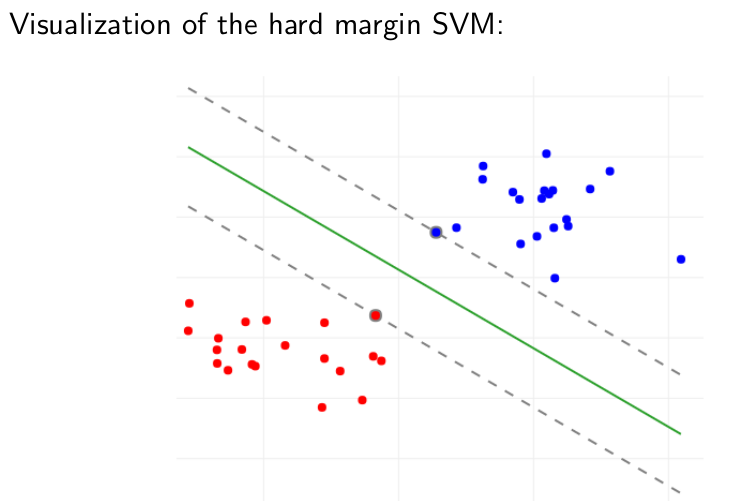
\includegraphics[scale=0.25]{svm1}

This is the \textit{hard margin} SVM problem in its usual form.
It is a nice convex optimization problem that we can solve in the usual way.

The Lagrangian is:
$$
L(w_0, w, \alpha) = \frac{1}{2}||w||^2 + \sum_{i=1}^n \alpha_i [1 - Y_i(\langle
w, x_i \rangle + w_0)]
$$

We compute the stationary points:

$$
\frac{\partial L}{\partial w} = \frac{\partial}{\partial w}
\left( \frac{1}{2}||w||^2 \right) + \frac{\partial}{\partial w}
\left(\sum_{i=1}^n \alpha_i \right) - \frac{\partial}{\partial w}\left( \sum_{i=1}^n \alpha_i Y_i \langle
w, x_i \rangle \right) - \frac{\partial}{\partial w} \left( \sum_{i=1}^n
\alpha_i Y_i w_0 \right)
$$
$$
w = \sum_{i=1}^n \alpha_i Y_i x_i
$$
$$
\frac{\partial L}{\partial w_0} = \frac{\partial}{\partial w_0}
\left( \frac{1}{2}||w||^2 \right) + \frac{\partial}{\partial w_0}
\left(\sum_{i=1}^n \alpha_i \right) - \frac{\partial}{\partial w_0}\left( \sum_{i=1}^n \alpha_i Y_i \langle
w, x_i \rangle \right) - \frac{\partial}{\partial w_0} \left( \sum_{i=1}^n
\alpha_i Y_i w_0 \right)
$$
$$
\sum_{i=1}^n \alpha_i Y_i = 0
$$
We plug them into the Lagrangian to obtain the dual. Let's proceed in steps. By
definition, $||v||^2 = \langle v, v \rangle$. So:

$$
\frac{1}{2} ||w||^2 = \frac{1}{2} \langle w, w \rangle = 
\frac{1}{2} \langle \sum_{i=1}^n \alpha_i Y_i x_i, \sum_{j=1}^n \alpha_j Y_j x_j \rangle
$$

The $\alpha$ and $Y$ are just scalars and so we can pull them out:

$$
= \frac{1}{2} \sum_{i=1}^n \sum_{j=1}^n \alpha_i \alpha_j Y_i Y_j \langle x_i, x_j \rangle
$$

Now we factor out the right hand side:
$$
\sum_{i=1}^n \alpha_i [1 - Y_i(\langle w, x_i \rangle + w_0)] = \sum_{i=1}^n
\alpha_i [1 - Y_i \langle w, x_i \rangle - Y_i w_0]
$$
$$
= \sum_{i=0}^n \alpha_i - \sum_{i=0}^n \alpha_i Y_i \langle w, x_i \rangle -
w_0 \sum_{i=0}^n \alpha_i Y_i
$$

We know that:
$$
w_0 \sum_{i=0}^n \alpha_i Y_i = w_0 \times 0 = 0
$$

Now let's plug $w$ into the middle term:

$$
\sum_{i=0}^n \alpha_i Y_i \langle \sum_{j=0}^n \alpha_j Y_j x_j, x_i \rangle
$$

Again we can pull out the scalars:

$$
= \sum_{i=0}^n \sum_{j=0}^n \alpha_i \alpha_j Y_i Y_j \langle x_i, x_j \rangle
$$

We recombine everything to form the dual:
$$
q(\alpha) = \frac{1}{2} \sum_{i=1}^n \sum_{j=1}^n \alpha_i \alpha_j Y_i Y_j
\langle x_i, x_j \rangle + \sum_{i=1}^n \alpha_i - 
\sum_{i=0}^n \sum_{j=0}^n \alpha_i \alpha_j Y_i Y_j \langle x_i, x_j \rangle
$$

$$
= \sum_{i=1}^n \alpha_i - \frac{1}{2} \sum_{i=0}^n \sum_{j=0}^n \alpha_i \alpha_j Y_i Y_j \langle x_i, x_j \rangle
$$

Hence, the dual problem is:
$$
\max_{\alpha \in \mathbb{R}^n} 
\sum_{i=1}^n \alpha_i - \frac{1}{2} \sum_{i=0}^n \sum_{j=0}^n \alpha_i \alpha_j Y_i Y_j \langle x_i, x_j \rangle
$$

subject to:

$$
\alpha_i \geq 0 \quad \forall i
$$
$$
\sum_{i=0}^n Y_i \alpha_i = 0
$$

The last constraint is for feasibility: if we didn't have it, $q$ could tend to
$- \infty$ by letting $w_0$ tend to $\pm \infty$. Since this is a feasible
problem, Slater's condition is met. The dual gap is 0. Solving the dual is
equivalent to solving the primal. 

KKT and slackness and support vectors?


\medskip

\textit{Soft margin}

The above approach may not always be possible (since it requires linear
seperability) or feasible (since it may lead to overfitting). So, we have the
alternative soft margin approach.

We introduce slack variables, as well as a cost parameter to control them. The
problem becomes:

\end{document}



Reminder: 3 methods
LDA
Logistics
SVM

Logistic regression
Bayes classifier is also linear classifier
MLE is equivalent to ERM with respect to linear hypothesis class and logistic
loss
Since logistic loss is convex function of margin y f(x)
Can add a regularizer, typically L1 or L2 - useful to prevent overfitting
If you have more d than n, can always achieve perfectly separate

LDA works poorly bc of squared loss in a classification problem - for squared
loss, points with large margin are penalized

SVM achieves data compression - solution depends ona  small subset of D, the
so-called support vectors

Have to look at both prime and dual
Write down Lagrangian - slide 37
Study SVM this weekend
Hard margin only if linearly separable (and even then might not want to bc of
danger of overfitting)

Soft margin - allow some observations to be incorrectly classified and/or inside
envelope
Bigger the C, the more tolerant you are to violations of envelope
Can show that that formulation equivalent to ERM

Dual allows non-linear decision boundary

When n is large, use primal
When d is large, use dual


